\documentclass[10pt,a4paper]{article}
\usepackage[utf8]{inputenc}
\usepackage[T1]{fontenc}
\usepackage[spanish]{babel}
\usepackage{amsmath}
\usepackage{amsfonts}
\usepackage{amssymb}
\usepackage{graphicx}
\usepackage{float}
\usepackage{multicol}
\usepackage[dvipsnames]{xcolor}
\usepackage{hyperref}
\definecolor{pinegreen}{rgb}{0.36, 0.54, 0.66}
\hypersetup{
    colorlinks=true,
    linkcolor=pinegreen,      
    urlcolor=red,
    }
\addto{\captionsspanish}{\renewcommand{\abstractname}{Abstract}}
\newcommand{\celda}[1]{
	\begin{minipage}{2cm}
		\vspace{2mm}
		#1
		\vspace{2mm}
	\end{minipage}
}
\definecolor{pinegreen}{rgb}{0.36, 0.54, 0.66}
\usepackage[left=2.00cm, right=2.00cm, top=2.00cm, bottom=2.00cm]{geometry}
\author{Gabriel Hernandez Bello}
\begin{document}
	
	\begin{figure}[H]
		\raggedright
		
\includegraphics[scale=0.2]{IMG/logo_udec.png} \hfill 
\includegraphics[scale=0.5]{IMG/cfm_logo.png}
	\end{figure}

	\vspace{6mm}
	%ESTE CENTER ES EXCLUSIVO PARA EL TITULO DEL PAPER, AUTOR Y UNIVER.
	\begin{center}
		{\Large \textbf{Medición de la altura del Campanil}}\\
		\vspace{2mm}
		{\large Gabriel Hernández Bello$^{1}$}\\
		\vspace{6.5mm}
		$^1$\textit{Universidad de Concepción, Facultad de Ciencias Físicas y Matemáticas, Ciencias Físicas. }\\
	\end{center}

	\begin{center}
		\textcolor{pinegreen}{\rule{150mm}{0.8mm}}
	\end{center}

      %ESTE ABSTRACT ES PARA EL RESUMEN PROPIAMENTE DICHO Y PARA LAS PALABRAS CLAVES (KEYWORDS) ,NOTA:el comando \par sirve para iniciar el nuevo parrafo con sangría.
	\begin{abstract}
		\underline{\textbf{Palabras Claves:}} \hspace{2mm} \textit{palabra1, palabra2, palabra3.}
	\end{abstract}
	
	\begin{center}
		\textcolor{pinegreen}{\rule{150mm}{0.8mm}}
	\end{center}
	
	\begin{multicols}{2}
		\section{Introducción}
			El campanil de la Universidad de Concepción es un campanario icónico de la universidad y la ciudad chilena de Concepción \cite{wikicamp}. Fue construido hacia 1943 gracias a la iniciativa de Enrique Molina Garmendia, quien apasionado por la Universidad de California, en Berkeley, esgrimía la idea de una \emph{ciudad universitaria} abierta para todos los visitantes y en la que se levantara un imponente campanil. El proyecto del campanil fue elegido del arquitecto Enrique San Martín y posteriormente construido bajo la suérvisión del Constructor Civil Juan Villa Luco. Se hizo de concreto armado, con 42 metros y 50 centímetros de altura, con escaleras en su interior y un balcón en la parte superior.\\
			En el presente laboratorio, usaremos herramientas matemáticas para calcular y verificar la altura del Campanil de la Universidad de Concepción.
		\section{Marco Teórico}
		\subsection{Trigonometría}
		La trigonometría es una rama de la matemática que se encarga de estudiar y medir los triángulos, las relaciones entre sus ángulos y lados, y las razones trigonométricas. Estas son de gran interés por su amplia aplicabilidad.\\
		Las razones entre los lados de un triángulo rectángulo son llamadas trigonométricas. Las principales son el \emph{seno, coseno} y la \emph{tangente}.\\
		\section{Procedimiento Experimental y Resultados}
		Para calcular la altura del Campanil, diseñamos un instrumento sencillo para medir ángulos, compuesto por un transportador, una regla, un hilo y un objeto pesado. De esta forma, apuntamos el instrumento hacia la cima del Campanil, lo que provoca que el hilo (tensado por el peso) se desplace de su posición de equilibrio, formando un ángulo que medimos con el transportador. Además, usamos una hunicha para medir la separación entre el Campanil y la posción donde se mide el ángulo. Luego, estimamos la altura del Campanil para distintas distancias usando la siguiente fórmula:
		\begin{equation}\label{Ec. altura}
		D = d + L \tan(\alpha).
		\end{equation}
		Donde $D$ representa la altura del campanil, $L$ la distancia entre campanil y el punto de medición del ángulo, $d$ la distancia entre la base del campanil y el punto de observación del ángulo y $\alpha$ el ángulo obtenido con el instrumento de medición.
		
		
		\begin{figure}[H]
			\centering
			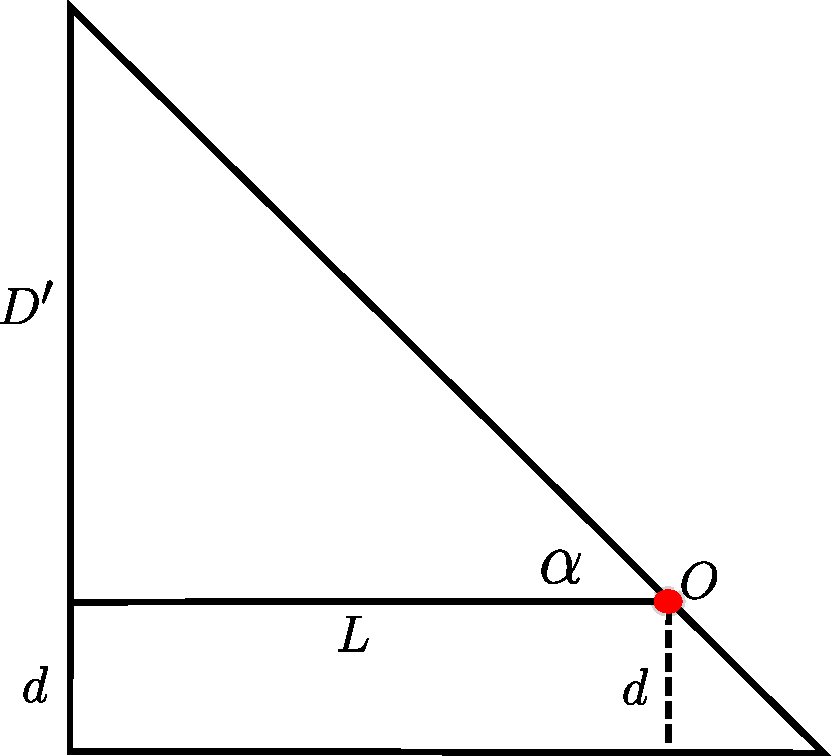
\includegraphics[scale=0.4]{IMG/camp.pdf} 
			\label{Diagrama campanil}
			\caption{Diagrama de la medición de la altura del campanil. Se respresenta $D^{\prime} = L \tan(\alpha)$,  $d$ la altura desde la base hasta el punto de observación del ángulo $O$ y $L$ la distancia entre el campanil y el punto de medición del ángulo.}
			\rule{80mm}{0.1mm}
		\end{figure}
		
	En la tabla \ref{tab:angulos_distancias.} se recogen los datos obtenidos para cuatro distancias y ángulos diferentes, donde se estimó el error de la altura del Campanil para cada medición de forma analítica con la siguiente fórmula:
		\begin{equation}
\sigma^{2} = \sigma_x^2 \left( \frac{\partial f}{\partial x} \right)^2 + \sigma_y^2 \left( \frac{\partial f}{\partial y} \right)^2 + \sigma_z^2 \left( \frac{\partial f}{\partial z} \right)^2 + ...
		\end{equation}
	\end{multicols}
	
	\begin{table}[H]
		\centering
		\begin{tabular}{|c|c|c|c|}
			\hline
			$\alpha$ (rad) & $L$ (m) & $d$ (m)&  $D$ (m) \\ \hline
			0.7850 $\pm$ 0.0087  & 40.0000 $\pm$ 0.0005 &  1.6000 $\pm$ 0.0005 & 41.57 $\pm$ 0.69\\ 
			0.7330 $\pm$ 0.0087 & 45.0000 $\pm$ 0.0005 & 1.6000 $\pm$ 0.0005 & 42.11 $\pm$ 0.70\\ 
			0.6810 $\pm$ 0.0087 & 50.0000 $\pm$ 0.0005 & 1.6000 $\pm$ 0.0005 &  42.08 $\pm$ 0.72\\ 
			0.6280 $\pm$ 0.0087 & 55.0000 $\pm$ 0.0005 & 1.6000 $\pm$ 0.0005 & 41.56 $\pm$ 0.73\\ \hline
		\end{tabular}
		\caption{Ángulos y Distancias Medidas}
		\label{tab:angulos_distancias.}
		\rule{100mm}{0.1mm}
	\end{table}

\begin{multicols}{2}
	\section{Análisis}
Los gráficos \ref{Grafico campanil} y \ref{Grafico campanil ajustado}  presentan los datos obtenidos durante el proceso experimental junto a su ajuste lineal, 		representado por la línea punteada. Del gráfico \ref{Grafico campanil} notamos que los datos se encuentran muy próximos entre si, 	con una desviación estándar de solo 0.31. Por ello, optamos por visualizar los datos en una escala más adecuada.  De esta forma, en el gráfico \ref{Grafico campanil ajustado} observamos que la aproximación lineal resulta en una linea recta con una pendiente aproximadamente nula, que estabiliza el valor de la altura del Campanil a 41.83 [m]. Esto es de esperarse, pues estamos comparando la altura del campanil para distintos valores del ángulo $\alpha$. . Por su parte, destacamos la elección de solo cuatro datos, pues son suficientes para ajustar una recta que pase por todos los puntos y sus respectivos errores.\\

Paralelamente, observamos que según la ecuación \ref{Ec. altura} el valor $D - d = L \tan(\alpha)$ es una constante, pues no variamos  $d$ durante el proceso experimental. Esto nos permite validar el comportamiento de los datos verificando que las variables $L$ y $\tan(\alpha)$ exhiben una relación inversamente proporcional. En efecto, en el gráfico \ref{Grafico de proporcionalidad} evidenciamos una relación lineal inversamente proporcional. Luego, concluimos que los datos obtenidos son coherentes.
	
	\begin{figure}[H]
		\centering
		\includegraphics[scale=0.5]{IMG/altura_1.pdf} 
		\caption{Gráfico de la altura del campanil para distintos valores del ángulo $\alpha$.}
		\label{Grafico campanil}
		\rule{80mm}{0.1mm}
	\end{figure}

	\begin{figure}[H]
		\centering
		\includegraphics[scale=0.5]{IMG/altura_2.pdf}
		\caption{Gráfico de la altura del campanil para distintos valores del ángulo $\alpha$ con los límites en el eje vertical adecuados.}
		\label{Grafico campanil ajustado}
		\rule{80mm}{0.1mm}
	\end{figure}
	
	\begin{figure}[H]
		\centering
		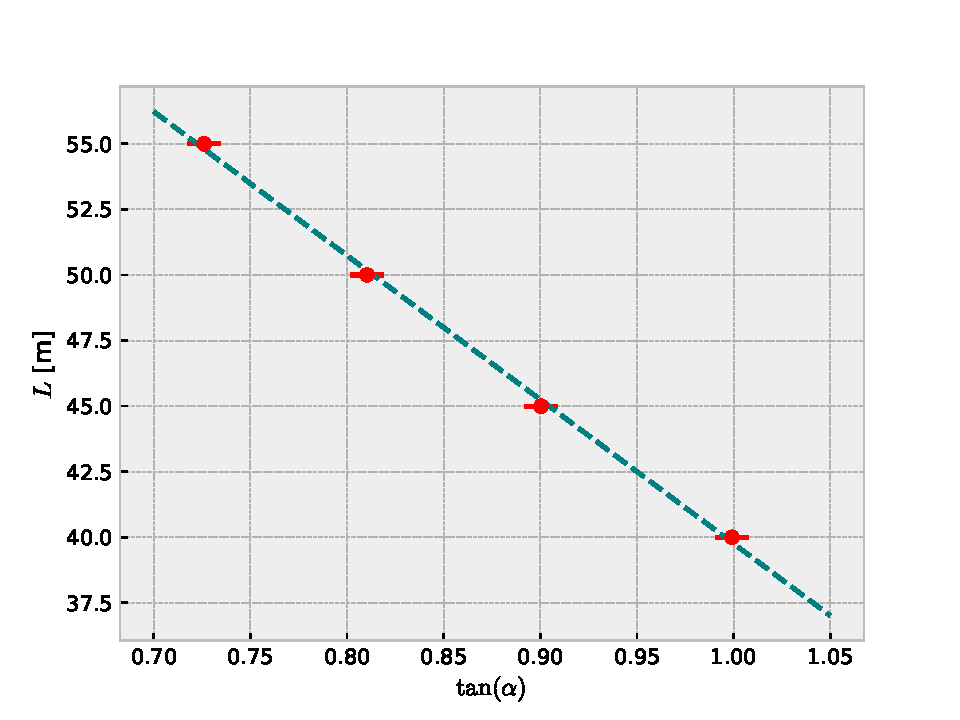
\includegraphics[scale=0.5]{IMG/proporcionalidad.pdf}
		\caption{Gráfico de la distancia entre el Campanil y el punto de observación $L$ respecto a la tangente del ángulo de elevación $\alpha$.}
		\label{Grafico de proporcionalidad}
		\rule{80mm}{0.1mm}
	\end{figure} 

En definitiva, considerando el valor promedio de los datos obtenidos y su desviación estándar, en este experimento estimamos la altura del Campanil $D$: $$D = 41.83 \pm 0.31 [m].$$

Ahora bien, la altura del Campanil es un dato conocido. Con ello, es posible calcular el error absoluto y porcentual de nuestra estimación, de esta forma:
\begin{align*}
\epsilon_{abs} &= |42.5[m] - 41.83[m]| = 0.67 [m]\\
\epsilon_{rel} &= \frac{0.67[m]}{41.83[m]}\cdot 100 = 1.6 \% 
\end{align*}
Mostrando así la proximidad de la estimación realizada en este experimento.
\section{Conlusión}
En el análisis, demostramos la efectividad del método empleado para estimar la altura del campanil, lo que se reflejó en el bajo error absoluto y relativo de la medición. Sin embargo, observamos que el valor real de la altura del campanil no se encuentra dentro del margen del valor estimado, lo cual atribuimos a la falta de precisión en el proceso experimental. A pesar de ello, los resultados obtenidos se acercan considerablemente al valor esperado, lo que destaca la gran capacidad y utilidad de las herramientas matemáticas utilizadas en la estimación.



		
	\end{multicols}
	
	\bibliographystyle{unsrt}
	\bibliography{ref}

\end{document}